% !TeX root=../main.tex
\قسمت{مقدمه}
ایستگاه هواشناسی، مرکزی مجهز به تجهیزات و ابزارهایی برای اندازه گیری‌های جوی است که به ارائه اطلاعات برای پیش بینی و مطالعه آب و هوا می‌پردازد. اندازه گیری های انجام شده معمولا شامل دما، فشار هوا، رطوبت، سرعت باد، جهت باد و مقدار بارش است. مشاهدات دستی حداقل یک بار در روز انجام می شود، در حالی که اندازه گیری های خودکار حداقل یک بار در ساعت انجام می‌پذیرد.

ایستگاه های هواشناسی معمولی مجهز به ابزارهای زیر هستند \مرجع{wikipedia:Weather_station}:

\شروع{فقرات}
\فقره
رطوبت‌سنج برای اندازه گیری رطوبت
\فقره
فشارسنج برای اندازه گیری فشار جو
\فقره 
دماسنج برای اندازه گیری دمای هوا
\فقره
پیرانومتر برای اندازه گیری تشعشعات خورشیدی
\فقره
باران‌سنج برای اندازه گیری میزان بارش باران در طی یک دوره زمانی مشخص
\فقره
تجهیزاتی نظیر بادسنج، پرچم باد یا جوراب باد برای اندازه گیری سرعت و جهت باد
\پایان{فقرات}

ایستگاه های پیشرفته تر همچنین ممکن است شاخص فرابنفش، رطوبت برگ، رطوبت خاک، دمای خاک، دمای آب در حوضچه ها، دریاچه ها، نهرها یا رودخانه ها و گاهی داده های دیگر را اندازه گیری کنند. به جز دستگاه‌هایی که نیازمند تماس مستقیم با عناصر مورد اندازه گیری هستند (نظیر بادسنج)، دیگر سنسورها و دستگاه‌ها باید در محفظه‌ای به دور از تابش مستقیم خورشید و وزش باد قرار بگیرند.

ایستگاه‌های هواشناسی سینوپتیک 24 ساعته به صورت خودکار هر سه ساعت به سه ساعت پارامتر‌های جوی را پس از اندازه‌گیری و جمع‌آوری از طریق شبکه‌های مخابراتی منتقل می‌کنند. به طور مشابه ایستگاه‌هایی با نام متار این کار را هر  یک ساعت انجام‌ می‌دهند. وظیفه این ایستگاه‌ها جمع‌آوری اطلاعات جوی از محدوده‌هایی وسیع و مخابره به ایستگاه‌های اصلی به منظور اطلاع از وضعیت حال و گذشته و پیش بینی شرایط آب و هوایی مناطق در آینده است. 

هدف این پروژه پیاده سازی نوعی ایستگاه هواشناسی سینوپتیک است که با تجهیزات ارزان و کم‌مصرف دیجیتالی پارامتر‌های جوی لازم را جمع آوری و به صورت بی‌سیم به ایستگاهی جهت ثبت و نمایش مخابره می‌کند. در این پروژه از میکروکنترلرهای \متن‌لاتین{ARM} سری \متن‌لاتین{STM32F10X} به عنوان هسته اصلی پردازش در هر دو سمت سنسور و ایستگاه و از ماژول لورا (\متن‌لاتین{LoRa}) با چیپ \متن‌لاتین{SX1278} به منظور برقراری ارتباط بی‌سیم استفاده می‌شود.

\قسمت{اجزای سیستم}

این سیستم به دو دستگاه اصلی تقسیم می‌شود، یک دستگاه جهت جمع آوری اطلاعات جوی برروی یک میله در ارتفاع 10 متری سطح زمین قرار می‌گیرد و اطلاعات جوی نظیر دما، رطوبت، فشار، شدت نور، سرعت و جهت باد را از سنسور‌های مربوطه جمع آوری کرده و به صورت بی‌سیم به دستگاه دیگر، که در ایستگاه اصلی قرار دارد، مخابره می‌کند؛ سپس اطلاعات دریافت شده در دستگاه دوم جهت ثبت و ذخیره به رایانه منتقل می‌شود. در اینجا به دستگاه اول که وظیفه جمع آوری اطلاعات جوی را دارد سنسور و دستگاه دوم که وظیفه دریافت اطلاعات مخابره شده و انتقال به رایانه را دارد ایستگاه می‌گوییم. بلوک دیاگرام کلی این سیستم و نحوه ارتباط بخش‌های مختلف با یکدیگر در شکل \رجوع{fig:systemDesign} آمده است.

\begin{figure}[!h]
	\centering
	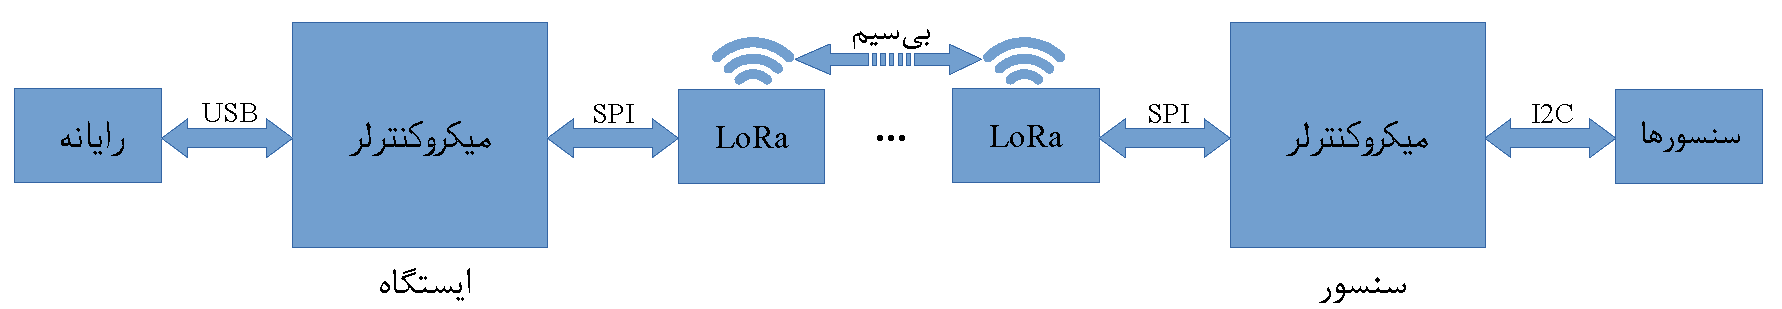
\includegraphics[width=\linewidth]{Assets/system design.pdf}
	\caption{بلوک دیاگرام اجزای سیستم و نحوه ارتباط اجزای مختلف با یکدیگر.}
	\label{fig:systemDesign}
\end{figure}

\زیرقسمت{میکروکنترلر}

هسته اصلی پردازش در هر دو سمت ایستگاه و سنسور میکروکنترلر \متن‌لاتین{STM32f103CBT6} انتخاب شده است که با توجه به موجود بودن در بازار ایران و دارا بودن 2 عدد \متن‌لاتین{I\بالانویس‌متنی{2}C}\پانویس{Inter-Integrated Circuit}، 2 عدد \متن‌لاتین{SPI}\پانویس{Serial Peripheral Interface}، اینترفیس \متن‌لاتین{USB}\پانویس{Universal Serial Bus} و 3 عدد تایمر 16 بیتی نیاز به حداقل 1 عدد \متن‌لاتین{I\بالانویس‌متنی{2}C} (در سمت سنسور)، 1 عدد \متن‌لاتین{SPI} (در هر دو سمت)، اینترفیس \متن‌لاتین{USB} (در سمت ایستگاه)  و 1 عدد تایمر (در سمت سنسور) را برآورده می‌کند. همچنین حالت \متن‌لاتین{Sleep} و واحد \متن‌لاتین{RTC} موجود در این میکروکنترلر‌ها به کاهش مصرف انرژی در وقفه‌های سه ساعته کمک می‌کند؛ به طوری که استفاده از سیستم باتری و پنل خورشیدی را ممکن می‌سازد.

\زیرقسمت{ارتباط بی‌سیم}
به طور کلی در این سیستم مصرف پایین انرژی به دلیل استفاده از سیستم باطری و پنل خورشیدی بسیار اهمیت دارد. استفاده از شبکه تلفن همراه\پانویس{The Global System for Mobile Communications (GSM)} به عنوان راه حلی ابتدایی برای ارتباط بی سیم، علاوه بر نداشتن صرفه اقتصادی مصرف انرژی زیادی را به سیستم تحمیل می‌کند. همچنین تضمینی برای وجود پوشش شبکه تلفن همراه در مناطقی که قرار است داده‌های جوی از آن جمع آوری شود وجود ندارد. ازین این رو بهترین رویکرد استفاده از گیرنده و فرستنده‌های رادیویی در باندهای فرکانسی بدون نیاز به مجوز (\متن‌لاتین{ISM}) است. از میان گزینه‌های موجود ماژول‌های لورا\پانویس{LoRa (Long Range)} به لطف مدولاسیون \متن‌لاتین{CSS\پانویس{Chirp Spread Spectrum}} که از آن بهره می‌برند دارای مصرف توان پایین، ناحیه پوشش وصیع و نفوذ پذیری مناسبی هستند که کاملا با نیازهای ما سازگار است. 

ماژول \متن‌لاتین{LoRa Ra-02} با تراشه \متن‌لاتین{Sx1278} دارای رنج فرکانسی 410 تا 525 مگاهرتز،و توان انتقالی ماکسیموم 18\متن‌لاتین{dBm} است و از مدولاسیون‌‌های \متن‌لاتین{LoRa}، \متن‌لاتین{FSK}\پانویس{Frequency Shift Keying} و \متن‌لاتین{OOK}\پانویس{On Off Keying} پشتیبانی می‌کند. برای ارتباط بی‌سیم در این سیستم از این ماژول استفاده شده است. 

\زیرقسمت{سنسورها} 

به منظور استخراج داده‌های جوی نظیر دمای هوا، رطوبت، فشار، شدت نور و... از سنسورهای دیجیتال استفاده می‌شود. این سنسورها علاوه بر کم مصرف بودن دارای دقت بالا و تاخیر پایینی در اندازه گیری پارامتر‌های مورد نظر هستند. با دارا بودن این ویژگی‌ها این سنسور‌ها کاملا با سیستم تغذیه باتری و سلول خورشیدی سازگار هستند.

\زیرزیرقسمت{فشارسنج}

تغییرات فشار جوی یکی از عناصر مهم در پیش بینی وضعیت آب و هوا است. فشارسنج‌های جیوه‌ای از اواخر قرن 16 جهت پیش بینی وضعیت آب و هوا مورد استفاده قرار می‌گرفت. به طور کلی تغییر فشار هوا رو به بالا نشان دهنده آسمان آفتابی، گرم و صاف و تغییر فشار هوا رو به پایین نشان دهنده بارش باران، طوفان و آسمانی مملو از ابر‌های باران‌زا است. علاوه بر این فشار هوا یکی از عوامل موثر در سنجش سرعت باد نیز به شمار می‌آید. 

سنسور استفاده شده برای این منظور ماژول سنسور \متن‌لاتین{BMP180} است که با مصرف جریان تنها در حد چند میکرو آمپر دقتی معادل با 0٫3 هکتو پاسکال دارد و در فشار هوا در بازه 300 تا 1100 هکتو پاسکال را اندازه‌گیری می‌نمایید. نحوه ارتباط با این ماژول از طریق رابط \متن‌لاتین{I\بالانویس‌متنی{2}C} است. 

\زیرزیرقسمت{شدت نور}

شدت نور خورشید یکی از پارامتر‌های اصلی سنجش وضعیت آب و هوا است. از این سنسور جهت نشخیص ابری یا آفتابی بودن هوا می‌توان استفاده کرد. همچنین به دلیل اهمیت سلامت پوست، معمولا در کنار این سنسور از سنسور سنجش شدت \متن‌لاتین{UV} به منظور اطلاع رسانی از شدت \متن‌لاتین{UV} نیز استفاده می‌شود. 

جهت سنجش شدت نور از ماژول سنسور \متن‌لاتین{MAX44009} استفاده شده است که با 0٫65 میکرو آمپر مصرف جریان در هنگام کارکرد شدت نور در بازه‌ی 0٫045 لوکس تا 188 هزار لوکس را اندازه گیری می‌کند. همچنین اینترفیس ارتباطی این ماژول رابط سریالی \متن‌لاتین{I\بالانویس‌متنی{2}C} می‌باشد.

\زیرزیرقسمت{قطب‌نما}

از آنجایی که این دستگاه در سمت سنسور معمولا در ارتفاع 10 متری زمین روی یک میله نصب می‌شود، قرار دادن دستگاه در جهت جغرافیایی خاص، به جهت سنجش جهت باد، ممکن است دشوار باشد (یا حتی خیلی دقیق نباشد). با وجود سنسور قطب‌نما در این دستگاه (برخلاف برخی دستگاه‌های مشابه) دیگر نیازی به نصب دستگاه در جهت جغرافیایی خاص نخواهد بود.

سنسور استفاده شده برای این منظور سنسور \متن‌لاتین{QMC5883L} است. که با ماکسیموم 100 میکرو آمپر جریان مصرفی میتوان به دقت یک تا دو درجه در جهت یابی رسید. همچنین طریقه ارتباط این سنسور با میکروکنترلر از طریق رابط \متن‌لاتین{I\بالانویس‌متنی{2}C} است.

\زیرزیرقسمت{دما و رطوبت هوا}

درکتار وضعیت آسمان (ابری، آفتابی، بارانی و... بودن) معمولا به طور مستقیم پارامتر دمای هوا نیز در اطلاع رسانی وضعیت و پیش بینی آب و هوا نقش ایفا می‌کند. در کنار این موارد رطوبت هوا نیز، علاوه بر نقشی که در پیش بینی دارد، معمولا به طور مستقیم به سمع و نظر مخاطبین می‌رسد. علاوه این رطوبت نسبی هوا در کنار دمای هوا نقش مهمی در رسیدن به آسایش حرارتی در بدن انسان (و موجودات) دارد. به طوری کلی در دمای هوای بالاتر به رطوبت نسبی کمتری نسبت به دمای هوای پایین تر برای رسیدن به سطح آسایش  حرارتی نیاز است \مرجع{Schiavon2013}. 

ماژول سنسور \متن‌لاتین{AHT10} دما و رطوبت نسبی هوا را با دقت 0٫01 درجه سلسیوس و 0٫024 درصد با تنها 3٫3 میکرو وات مصرف توان اندازه‌گیری می‌کند. همچنین این ماژول در رطوبت 0 تا 100 درصد و دمای  40- تا 100 درجه‌ی سلسیوس قابل استفاده است. خروجی این ماژول نیز سیگنال دیجیتال ارتباطی \متن‌لاتین{I\بالانویس‌متنی{2}C} است. 

\زیرزیرقسمت{شدت و جهت باد}

روش‌های مختلفی برای سنجش شدت باد وجود دارد، عمدتا در این کاربرد دو روش سنجش مکانیکی و آلتراسونیک مورد استفاده قرار می‌گیرد. در سنجش شدت و جهت باد در روش مکانیکی از دو ابزار به صورت مستقل (در برخی موارد این دو ابزار در قالب یک دستگاه در کنار هم قرار میگیرند)، یک ابزار برای سنجش شدت و ابزاری دیگر برای تعیین جهت، امورد استفاده قرار می‌گیرد. هر دو دستگاه دارای قطعات متحرک اند و یکی با داشتن پره‌هایی شبیه به دم هلی کوپتر با وزرش باد در جهت وزش قرار میگیرد و دیگری دارای پره‌هایی است که با وزش باد پره‌ها همانند پره‌های توربین به حدکت در می‌آید که با توجه به سرعت چرخش پره‌ها سرعت باد قابل اندازه‌ گیری است. در اندازه‌گیری‌های این دستگاه‌ها محدودیت‌هایی وجود دارد و اغلب این نوع ابزارها در وزش باد ملایم عملکرد صحیحی از خود نشان نمی‌دهند. همچنین در اندازه گیری زاویه وزش ممکن اند محدود به زوایای خاصی باشند. 

در روش اندازه‌گیری شدت و جهت باد با آلتراسونیک اندازه‌گیری‌ها می‌تواند در قالب تنها یک دستگاه ،بدون قطعات متحرک و با دقتی بالاتر انجام پذیرد. در این روش 2 فرستنده و گیرنده آلتراسونیک همان طور که در شکل \رجوع{fig:oneAxisUltrasonic} نشان داده شده است روبروی یکدیگر در فاصله‌ مشخص $d$ قرار داده می‌شوند.

\begin{figure}[!h]
	\centering
	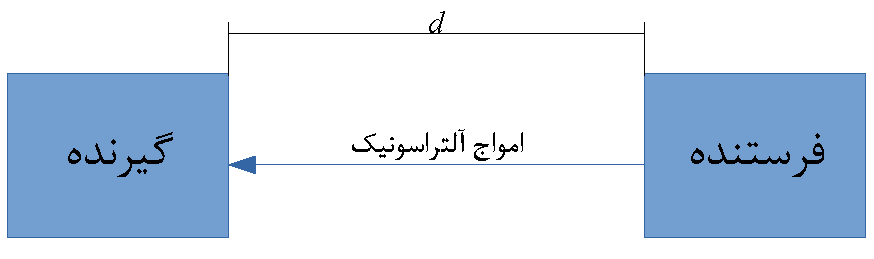
\includegraphics[width=0.6\linewidth]{Assets/ultrasonic one axis.pdf}
	\caption{نحوه قرار گیری فرستنده و گیرنده آلتراسونیک.}
	\label{fig:oneAxisUltrasonic}
\end{figure}

فرستنده امواج صوتی با فرکانس 40 کیلو هرتز تولید می‌کند. فاصله زمانی بین ارسال امواج صوتی از فرستنده و دریافت این امواج در گیرنده اندازه‌گیری می‌شود. با توجه به رابطه \رجوع{eq:speed} سرعت $v$ با داشتن با داشتن فاصله $d$ و زمان تاخیر بین ارسال موج صوتی در فرستنده و دریافت آن در گیرنده  $t$ قابل اندازه گیری است.
\begin{equation}\label{eq:speed}
	v = \frac{d}{t}
\end{equation}

سرعت $v$ بدست آمده از این رابطه مطابق رابطه \رجوع{eq:expandSpeed} متشکل از سرعت صوت $v_s$ و سرعت باد $v_{wx}$  است \مرجع{7988049}.
\begin{equation}\label{eq:expandSpeed}
	v = v_s + v_{wx}
\end{equation}

در صورتی که وزش باد در جهت موافق حرکت امواج صوتی باشد زمان تاخیر در دریافت امواج نسبت به حالی که باد نوزد کمتر شده و در نتیجه سرعت $v$ نسبت به حالتی که باد نوزد افزایش می‌یابد (یعنی علامت $v_{wx}$ مثبت بوده و $v = v_s+v_{wx}$). در صورتی که وزش باد در خلاف جهت حرکت امواج صوتی باشد زمان تاخیر در دریافت امواج نسبت به حالتی که باد نوزد بیشتر شده و در نتیجه سرعت $v$ کاهش می‌یابد (یعنی علامت $v_{wx}$ منفی بوده و $v = v_s-v_{wx}$). با داشتن سرعت صوت $v_s$، فاصله $d$ و محاسبه زمان $t$ میتوان با توجه به معادلات \رجوع{eq:speed} و \رجوع{eq:expandSpeed} سرعت باد $v_{wx}$ و جهت باد (علامت سرعت $v_{wx}$) روی یک محور مطابق رابطه \رجوع{eq:speedWindX} بدست آورد. 

\begin{equation}\label{eq:speedWindX}
	v_{wx} = \frac{d}{t} - v_s
\end{equation}

به منظور سنجش شدت و جهت باد در دو بعد می‌توان دو فرستنده و گیرنده دیگر برروی محوری عمود بر محور متصل کننده فرستده و گیرنده فعلی قرار داد و با محاسبه دو بردار سرعت، بردار سرعت برآیند را بدست آورد.

\begin{figure}[!h]
	\begin{subfigure}[b]{0.5\textwidth}
		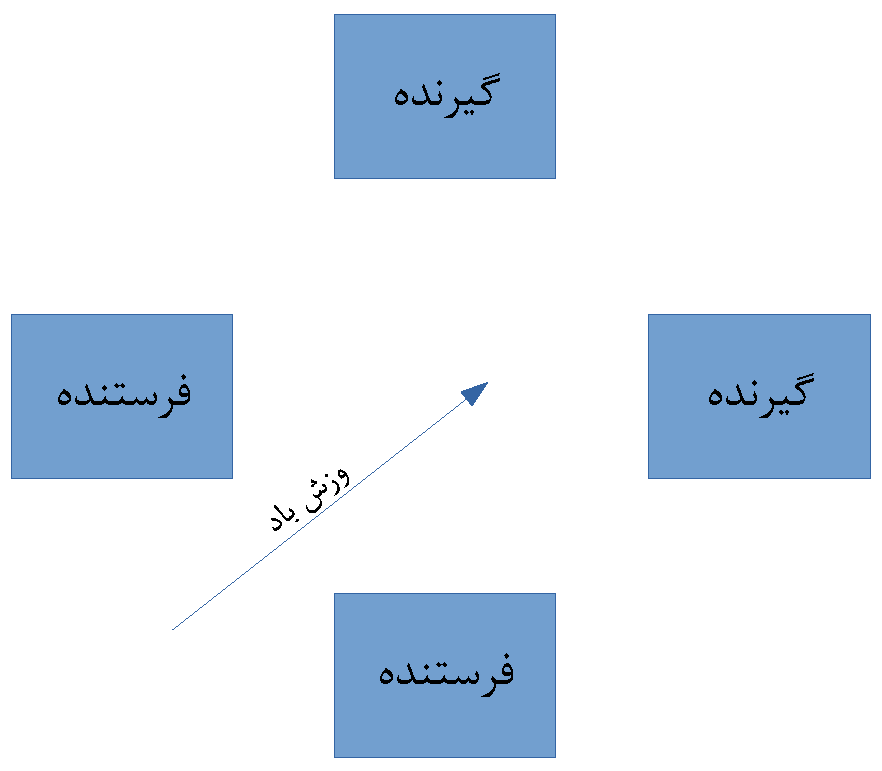
\includegraphics[width=\linewidth]{Assets/ultrasonic 2d.pdf}
		\caption{}
		\label{fig:2dUltrasonic}
	\end{subfigure}
	\begin{subfigure}[b]{0.5\textwidth}
		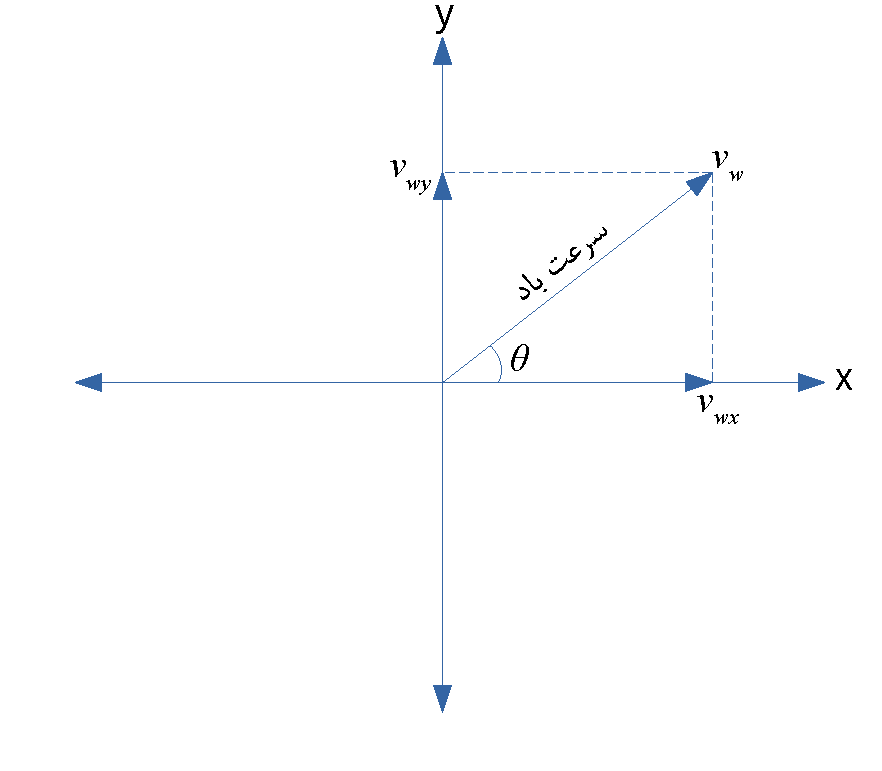
\includegraphics[width=\linewidth]{Assets/ultrasonic 2d axis.pdf}
		\caption{}
		\label{fig:2dUltrasonicAxis}
	\end{subfigure}
	\caption{نحوه قرار گیری فرستنده و گیرنده آلتراسونیک دو محوره و نمودار متناظر با آن‌ها.}
\end{figure}

اگر نحوه قرار گیری فرستنده و گیرنده‌ها مطابق شکل \رجوع{fig:2dUltrasonic} باشد در این صورت صفحه مختصات متناظر با آن مطابق شکل \رجوع{fig:2dUltrasonicAxis} خواهد بود. اندازه $v_w$ و زاویه $\theta$ بردار سرعت باد از طریق روابط \رجوع{eq:windSpeed} بدست می‌آیند.

\begin{equation}\label{eq:windSpeed}
	\begin{split}
		v_w = \sqrt{v_{wx}^2 + v_{wy}^2}\\
		\theta = \tan^{-1}{\left( \frac{v_{wy}}{v_{wx}}\right)}
	\end{split}	
\end{equation}

\begin{table}[!t]
	\centering
	\caption{ضرایت  محاسبه سرعت صوت (فرمول \رجوع{eq:soundSpeed})}
	\label{tb:speedOfSoundcoefficients}
	\begin{tabular}{cc}
		\hline \hline
		 ضرایب & \\
		\hline
		$a_{0}$ & $331.5024$ \\
		$a_{1}$ & $0.603055$ \\
		$a_{2}$ & $-0.000528$ \\
		$a_{3}$ & $51.471935$ \\
		$a_{4}$ & $0.1495874$ \\
		$a_{5}$ & $-0.000782$ \\
		$a_{6}$ & $-1.82 \times 10^{-7}$ \\
		$a_{7}$ & $3.73 \times 10^{-8}$ \\
		$a_{8}$ & $-2.93 \times 10^{-10}$ \\
		$a_{9}$ & $-85.20931$ \\
		$a_{10}$ & $-0.228525$ \\
		$a_{11}$ & $5.91 \times 10^{-5}$ \\
		$a_{12}$ & $-2.835149$ \\
		$a_{13}$ & $-2.15 \times 10^{-13}$ \\
		$a_{14}$ & $29.179762$ \\
		$a_{15}$ & $0.000486$ \\
		\hline
	\end{tabular}
\end{table}

سرعت صوت $v_s$ به عنوان تابعی از دما، فشار و کسر مولی رطوب و کربن دی اکسید، با استفاده از رابطه \رجوع{eq:soundSpeed} قابل محاسبه است \مرجع{cramer1993variation}. ثوابت$a_1$ تا $a_{15}$ در جدول \رجوع{tb:speedOfSoundcoefficients} آمده اند.

\begin{equation}\label{eq:soundSpeed}
	\begin{aligned}
		v_s\left(\tau, p, x_w, x_{c}\right)=& a_{0}+a_{1} \tau+a_{2} \tau^{2}+\left(a_{3}+a_{4} \tau+a_{5} \tau^{2}\right) x_{w} \\
		&+\left(a_{6}+a_{7} \tau+a_{8} \tau^{2}\right) p+\left(a_{9}+a_{10} \tau+a_{11} \tau^{2}\right) x_{c} \\
		&+a_{12} x_{w}^{2}+a_{13} p^{2}+a_{14} x_{c}^{2}+a_{15} x_w p x_c
	\end{aligned}
\end{equation}

که $\tau$ دمای هوا (برحسب درجه سلسیوس)، $p$ فشار هوا (بر حسب پاسکال)، $x_w$ کسر مولی بخار آب در هوا و $x_c$ کسر مولی کربن دی‌اکسید در هوا است. $x_c$ را ثابت و برابر $400 \times 10^{-6}$ در نظر می‌گیریم. کسر مولی بخار آب در هوا $x_w$ از رابطه \رجوع{eq:x_w} بدست می‌آید \مرجع{rasmussen1997calculation}. 

\begin{equation}\label{eq:x_w}
	x_w=\frac{h f p_{sv}}{100 p}
\end{equation}

که $h$ درصد رطوب هوا، $p_{sv}$ فشار اشباع بخار آب در هوا و $f$ ضریب تقویت است و از طریق روابط 
\رجوع{eq:f} و \رجوع{eq:p_sv} محاسبه می‌شوند \مرجع{davis1992equation}.

\begin{equation}\label{eq:f}
	f=1.00062+3.14 \times 10^{-8} p+5.6 \times 10^{-7} \tau^{2}
\end{equation}
\begin{equation}\label{eq:p_sv}
	\begin{aligned}
		p_{s v}=& \exp \left(1.2811805 \times 10^{-5} T^{2}-1.9509874 \times 10^{-2} T\right.\\
		&\left.+34.04926034-6.3536311 \times 10^{3} / T\right)
	\end{aligned}
\end{equation}

که در این روابط $T$ دمای محیط بر حسب کلوین است، یعنی:
\begin{equation}
	T = \tau + 273.15
\end{equation}

\قسمت{پروتکل‌های ارتباطی}

قطعات الکترونیک نیز همانند انسان‌ها برای ارتباط با یکدیگر باید از یک زبان واحد قابل فهم برای هر دو طرف استفاده کنند که به این زبان ها پروتکل‌های ارتباطی گفته می‌شود. در این پروژه نیز همانند اکثر پروژه‌های الکترونیکی از تعدادی از این پروتکل‌ها برای برقراری ارتباط بین قطعات الکترونیکی مختلف (سنسور‌ها، فرستنده-گیرنده‌های رادیویی و میکروکنترلر) استفاده شده است. در زیر اطلاعات کلی هر یک از پروتکل‌های ارتباطی استفاده شده در این پروژه آمده است.

\زیرقسمت{پروتکل \متن‌لاتین{SPI}}

این پروتکل یک رابط ارتباط سریالی سنکرون (همزمان) چهار سیمه است که برای ارتباط بین تنها یک \متن‌لاتین{master} و چندین \متن‌لاتین{slave} می‌تواند مورد استفاده قرار گیرد. خطوط ارتباطی بین \متن‌لاتین{master} و \متن‌لاتین{slave} شامل خط سیگنال کلاک (\متن‌لاتین{SCLK}\پانویس{Serial Clock})، خط ارسال داده از \متن‌لاتین{master} به \متن‌لاتین{slave} (\متن‌لاتین{MOSI}\پانویس{Master Out Slave In})، خط ارسال داده از \متن‌لاتین{slave} به \متن‌لاتین{master} (\متن‌لاتین{MISO}\پانویس{Master In Slave Out}) و خط انتخاب \متن‌لاتین{slave} (\متن‌لاتین{SS}\پانویس{Slave Select} یا \متن‌لاتین{CS}\پانویس{Chip Select}). در حالت \متن‌لاتین{Full Duplex} به ازای هر \متن‌لاتین{slave} معمولا نیاز به یک پین انتخاب‌گر (\متن‌لاتین{SS} یا \متن‌لاتین{CS}) مجزا در سمت \متن‌لاتین{master} خواهد بود. 

\begin{figure}[!h]
	\centering
	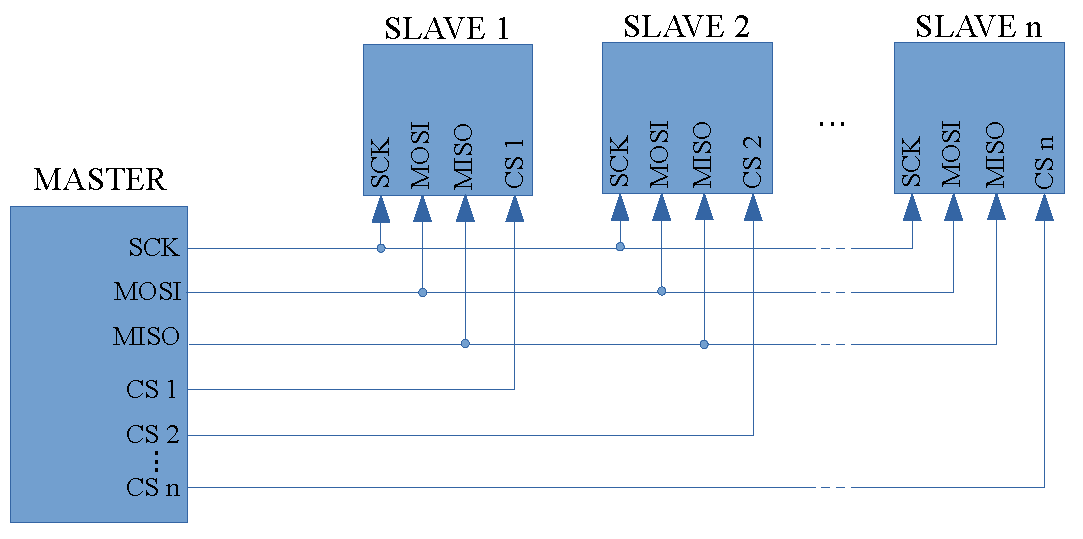
\includegraphics[width=.7\linewidth]{Assets/SPI.pdf}
	\caption{نحوه اتصال \متن‌لاتین{slave}ها به \متن‌لاتین{master}}
	\label{fig:SPIWiring}
\end{figure}

سیگنال کلاک همواره توسط \متن‌لاتین{master} تولید می‌شود و به ازای هر سیگنکال کلاک یک بیت داده منتقل می‌شود. از این رو ارسال داده از \متن‌لاتین{slave} به \متن‌لاتین{master} به طور تصادفی و در هر لحظه ممکن نیست و تنها \متن‌لاتین{slave} می‌تواند در لحظاتی که \متن‌لاتین{master} درخواست می‌کند و سیگنال کلاک اضافی را تولید می‌کند داده را برروی خط \متن‌لاتین{MISO} ارسال کند. البته به دلیل وچود خطوط مجزای ارسال و دریافت داده ارسال و دریافت همزمان داده نیز ممکن است. همچنین در این پروتکل \متن‌لاتین{slave}ها به تنهایی نمیتوانند با یکدیگر ارتباط برقرار کنند.

به جهت ارسال داده، \متن‌لاتین{master} از طریق قراردادن خط \متن‌لاتین{SS} (یا \متن‌لاتین{CS}) در حالت \متن‌لاتین{low} انتخاب می‌کند که با کدام \متن‌لاتین{slave} می‌خواهد ارتباط برقرار کند و همین وضعیت این خط را تا پایان فرآیند ارسال و دریافت داده در همین وضعیت (\متن‌لاتین{low}) نگهمیدارد. در همین حین سیگنال کلاک را روی خط \متن‌لاتین{SCLK} متناسب با طول داده ارسالی قرار می‌دهد (ماکسیموم فرکانس کلاک بستگی به ماکسیموم مقدار قابل شناسایی توسط \متن‌لاتین{slave} دارد) و داده ارسالی را نیز متناسب با کلاک روی خط \متن‌لاتین{MOSI} قرار می‌دهد (قرار دادن داده روی لبه بالارونده یا پایین رونده و همچنین ارسال از بیت \متن‌لاتین{MSB} یا \متن‌لاتین{LSB} بستگی به \متن‌لاتین{slave} دارد)؛ اگر قرار باشد \متن‌لاتین{slave} دیتایی در پاسخ به دیتای دریافتی ارسال کند (این امر باید از قبل مشخص باشد چرا که همان‌طور که گفته شد مسئول تولید کلاک فقط \متن‌لاتین{master} است) باید \متن‌لاتین{master} کلاک‌ها اضافی متناسب با دیتای مورد انتظار برای دریافت را روی خط \متن‌لاتین{SCLK} تولید کند و دیتای مربوطه را از روی خط \متن‌لاتین{MISO} بخواند.

\زیرقسمت{پروتکل \متن‌لاتین{I\بالانویس‌متنی{2}C}}

پروتکل \متن‌لاتین{I\بالانویس‌متنی{2}C} رابط سریالی سنکرون چند \متن‌لاتین{master} چند \متن‌لاتین{slave} دو سیمه است. این پروتکل برخلاف \متن‌لاتین{SPI} از سیستم‌ها دارای چند \متن‌لاتین{master} نیز پشتیبانی می‌کند (البته \متن‌لاتین{master}ها قادر به برقراری ارتباط با یکدیگر نیستند و از خطوط باس به طور همزمان نمی‌توانند استفاده کنند). در این پروتکل برای ارتباط از تنها دو خط سیگنال کلاک (\متن‌لاتین{SCL}\پانویس{Serial Clock Line}) و سیگنال دیتا (\متن‌لاتین{SDA}\پانویس{Serial Data Line}) استفاده می‌شود. در این پروتکل نیز سیگنال کلاک توسط \متن‌لاتین{master} کنترل می‌شود. اعلام شروع ارسال داده با بالا نگهداشتن خط \متن‌لاتین{SCL} و پایین کشیدن خط \متن‌لاتین{SDA} انجام می‌شود. اگر دو \متن‌لاتین{master} به طور همزمان قصد تبادل داده با \متن‌لاتین{slave}ها را داشته باشند هر کدام که زود تر \متن‌لاتین{SDA} را پایین بکشید اجازه استفاده از خط را دارد و \متن‌لاتین{master} دیگر باید تا پایان تبادلات \متن‌لاتین{master} اول صبرکند.

برای انتقال داده پس از اعلام شروع ارسال توسط \متن‌لاتین{master}، 7 بیت آدرس \متن‌لاتین{slave} که قرار است با آن ارتباط برقرار شود ارسال می‌شود و پس از آن یک بیت \متن‌لاتین{read/write} ارسال می‌شود تا \متن‌لاتین{slave} از قصد \متن‌لاتین{master} برای خواندن (سطح منطقی 1) یا نوشتن (سطح منطقی 0) مطلع شود (آدرس 10 بیتی نیر وجود دارد که نحوه ارسال آن کمی متفاوت است ولی فرآیند‌های دیگر در دریافت و ارسال داده یکسان است). در تمام طول ارسال و دریافت داده سیگنال کلاک نیز به طور منظم روی خط \متن‌لاتین{SCL} تولید می‌شود. بعد از ارسال آدرس توسط \متن‌لاتین{master}، \متن‌لاتین{slave}ها آدرس ارسالی را با آدرس خود مقایسه کرده و در صورتی که با آن مطابقت داشت بیت تصدیق (\متن‌لاتین{ACK}) را با پایین کشیدن \متن‌لاتین{SDA} تا قبل از کلاک نهم ارسال می‌کند. اگر بیت تصدیق در این زمان ارسال نشود و \متن‌لاتین{SDA} در سطح \متن‌لاتین{high} بماند ارسال داده متوقف می‌شود چرا که عدم دریافت بیت تصدیق نشان دهنده عدم وجود \متن‌لاتین{slave} مورد نظر روی خط و یا عدم توانایی \متن‌لاتین{slave} در رمزگشایی داده ارسالی است. 

پس از ارسال آدرس و دریافت تصدیق از سمت \متن‌لاتین{slave} با توجه به بیت \متن‌لاتین{read/write} ارسالی، داده توسط \متن‌لاتین{slave} (درحالت خواندن) و یا \متن‌لاتین{master} (در حالت نوشتن) روی خط \متن‌لاتین{SDA} قرار داده می‌شود. بعد از ارسال هر 8 بیت داده نیز لازم است بیت تصدیق دریافت داده‌ها (\متن‌لاتین{ACK}) از طرف دریافت کننده داده‌ها ارسال شود. بعد از ارسال یا دریافت تمام داده‌ها باید وضعیت توقف اعلام شود تا دیگر \متن‌لاتین{master}ها بتوانند پس از آن از خط استفاده کنند. اعلام وضعیت توقف با یک تغییر وضعیت \متن‌لاتین{SDA} از سطح منطقی 0 به 1 و پس از آن یک تغییر وضعیت از سطح منطقی 0 به 1  روی خط \متن‌لاتین{SCL} انجام می‌شود.

\زیرقسمت{USB}

پروتکل یو‌اس‌بی (\متن‌لاتین{USB}) یک پروتکل ارتباطی سریال آسنکرون (نا‌همزمان) دو سیمه است که ارتباطی بین چندین دستگاه‌ جانبی یا دیوایس (\متن‌لاتین{Device}) و دستگاه اصلی یا هاست (\متن‌لاتین{Host}) را فراهم می‌کند. یواس‌بی توسط یک گروه متشکل از شرکت‌های فعال در زمینه رایانه و الکترونیک ایجاد شد که هدف ساخت پروتکل سریال همه منظوره برای اتصال لوازم جانبی به رایانه را داشتند. به دلیل همه منظوره بودن یو‌اس‌بی استفاده از این پروتکل دارای جزئیات بسیار زیادی است و بر خلاف دو پروتکل قبلی راه اندازی این پروتکل ممکن است زمان بر باشد. در این پروژه از این پروتکل برای ارتباط دستگاه سمت ایستگاه با رایانه و همچنین تامین تغذیه آن استفاده می‌شود.

به طور کلی ارتباط بادیوایس با هاست نیازمند دارا بودن دیوایس کلاس (\متن‌لاتین{Device Class}) مشخص و شناخته شده‌ برای هاست است. پیاده سازی دیوایس کلاس‌های اختصاصی به خاطر پیچیدگی‌هایی که این پروتکل دارد امری بسیار زمان‌بر خواهد بود به همین دلیل معمولا استفاده از دیوایس کلاس‌ و لایبرری‌های متناطر با آن برای ساخت دستگاه‌های جدید مناسب ترین روش ممکن است (این کار همچنین امر دریافت گواهی‌های سخت افزاری و نرم‌افزاری یو‌اسی‌بی را نیز تسهیل می‌کند).

در این پروتکل 4 نوع انتقال داده وجود دارد. انتقال \متن‌لاتین{Control} که تنطیمات و مشخصات دستگاه و دستورات را منتقل می‌کند. انتقال \متن‌لاتین{Isochronous} که برای انتقال داد‌ه‌هایی که زمان بندی در آنها اهمیت دارد نظیر صدای میکروفون و تصویر وب کم مورد استفاده قرار میگیرد. انتقال \متن‌لاتین{Bulk} که برای ارسال داده‌های حجیم تر به صورت یکجا مورد استفاده قرار می‌گیرد مانند انتقال تصویر برای پرینت و یا اسکن و یا انتقال داده‌های ذخیره شده روی یک فلش مموری. انتقال \متن‌لاتین{Interrupt} که داده‌هایی با حجم بسیار کم و اهمیت زیاد را جابجا می‌کند که معمولا توسط موس ، کیبرد و جواستیک (\متن‌لاتین{Joystick}) و عموما در کلاس \متن‌لاتین{HID}\پانویس{Human interface device} استفاده می‌شود.

همان طور که گفته شد در این پروتکل لازم است دستگاه هاست از تمامی جزئیات کارکرد و مشخصات دستگاه دیواس مطلع شود. مشخصات کلی دستگاه مثل ورژن یو‌اس‌بی مورد استفاده، شناسه ونام سازنده، شناسه ونام دستگاه و مشخصات کلاس دستگاه در بخشی با عنوان \متن‌لاتین{Device Descriptor} با فرمتی خاص و مشخص به اطلاع رایانه می‌رسد. بخش دیگری با عنوان \متن‌لاتین{Configuration Descriptors} بیان کننده نحوه تغذیه و ماکسیموم توان مورد نیاز دستگاه متصل به یو اس بی است. بخش \متن‌لاتین{Interface Descriptors} نیز بیان کننده ویژگی‌های کلاس دستگاه است و شامل چندین \متن‌لاتین{Endpoint Descriptors} می‌شود که برای انجام آن ویژگی‌ها مورد نیاز اند. برای هر اندپوینت (\متن‌لاتین{Endpoint}) در سمت دیوایس از نظر سخت افزاری معمولا یک رجیستر یا مموری تعریف می‌شود که که دیتا با توجه به مشخات هر اندپوینت از آن خوانده می‌شود یا در آن نوشته می‌شود هر اند پوینت فقط مسئول یکی از اعمال خوانده شدن یا نوشته شدن است و برای هر دو عمل خواندن و نوشتن به دو اند پوینت نیاز است. ماکسیموم میتوان 16 اندپوینت تعریف کرد، اندپوینت 0 رزرو و برای مشخصات کنترلی استفاده می‌شود دیگر اندپوینت‌ها را می‌توان با مشخات مورد نیاز تعریف کرد. به طور مثال در این پروژه از کلاس \متن‌لاتین{CDC}\پانویس{Communications Device Class} استفاده شده است (که کلاس مورد استفاده در کارت‌های شبکه و مودم‌ها نیز هست). برای تبادل داده با رایانه در این کلاس از ارسال نوع بالک (\متن‌لاتین{Bulk}) استفاده می‌شود. پس اینترفیسی از نوع سی‌دی‌سی (\متن‌لاتین{CDC}) با اندپوینتی با دیتاتایپ بالک به عنوان ورودی و اندپوینتی دیگیر با دیتاتایپ بالک به عنوان خروجی باید داشته باشد. آدرس اندپوینت ورودی 0x01 و اندپوینت خروجی 0x81 تنظیم شده اند. همچنین چون قصد استفاده از یو‌اس‌بی در حالت فول اسپید (Full Speed) را داریم ماکسیموم سایز بسته ارسالی نیز 64$\times$1 بایت ذکر شده است. 

\قسمت{پیاده سازی سیستم}



\قسمت{نتایج}



\قسمت{نتیجه‌گیری}


